\section{Analyse}
\label{sec:analyse}
Nachdem ein geeigneter Datensatz erfasst wurde, können die Daten analysiert werden.
Für die Analyse gibt es zwei wesentliche Herangehensweisen: die Betrachtung von Korrelationsmaßen und Erstellung von Klassifikatoren.
Korrelationsmaße drücken aus, wie die Software-Metriken mit Sicherheitslücken zusammenhängen.
Klassifikatoren entscheiden anhand der Metriken, ob eine Komponente wahrscheinlich anfällig ist oder nicht.
Zuvor sollte festgelegt werden, welche Metriken für die Analyse verwendet werden sollen.
% Informational approach (Wo fließen Daten hin?) vs. structual approach (Wer ruft wen auf?)

\subsection{Wahl der Metriken}
Die Auswahl der Metriken ist vielfältig.
Alves et al. berechnen insgesamt 27 Metriken für Funktionen.
Einige davon sind CCC-Metriken, andere beziehen sich auf die Anzahl der Codezeilen oder auf das Verhältnis von Quellcode-Kommentaren zu Codezeilen.
In der Studie von Chowdhury und Zulkernine werden 21 Metriken berechnet~\cite{chowdhury_zulkernine_2009}.
Abbildung \ref{table1} zeigt einen Ausschnitt aus der Arbeit von Chowdhury und Zulkernine~\cite{chowdhury_zulkernine_2010}.
Zu sehen sind die englische Bezeichnungen und Beschreibungen für die Komplexitätsmetriken.

\begin{table}
	\caption{Tabelle mit den verwendeten Metriken~\cite{chowdhury_zulkernine_2010}}
	\label{table1}
	\begin{tabular}{|p{1.6cm}|p{10.4cm}|}
		\hline
		\textbf{Metrics} & \textbf{Description and Rationale} \\
		\hline
		McCabe's & McCabe's cyclomatic complexity: the number of independent paths through a program unit (i.e., number of decision statements plus one).
		For a file or class, it is the average cyclomatic complexity of the functions defined in the file or class. The higher this metric the more likely
		an entity is to be difficult to test and maintain without error.\\
		\hline
		Modified & Modified cyclomatic complexity: identical to cyclomatic complexity except that each case statement is not counted; the entire switch statement counts as 1.\\
		\hline
		Strict & Strict cyclomatic Complexity: identical to cyclomatic complexity except that the AND (\&\& in C/C++) and OR (||in C/C++) logical operators are also counted as 1.\\
		\hline
		Essential & Essential cyclomatic complexity: a measure of the code structuredness by counting cyclomatic complexity after iteratively replacing all structured programming primitives with a single statement.\\
		\hline
		Nesting & Nesting complexity: the maximum nesting level of control constructs (if, while, for, switch, etc.) in the function. Highly nested control	structures might make a program entity complex and hence difficult to comprehend by a programmer.\\
		\hline
		SLOC & Source Line Of Code: the number of executable lines of source code. Although SLOC measures size, prior research has found that SLOC highly correlates with complexity.\\
		\hline
		NOC & Number Of Children (NOC): the number of immediate sub-classes of a class or the count of derived classes. If class CA inherits class CB, then	CB is the base class and CA is the derived class. In other words, CA is the children of class CB, and CB is the parent of class CB. NOC measures inheritance complexity.\\
		\hline
		CBC & Count of Base Classes: the number of base classes. Like NOC, CBC measures inheritance complexity.\\
		\hline
	\end{tabular}
\end{table}

\subsection{Korrelationsmaße}
Zur Überprüfung der Hypothesen eigen sich Korrelationsmaße.
Die Behebung einer Sicherheitslücke müsste eine Verbesserung der CCC-Metriken nach sich ziehen.
Ein mögliches Maß für die Korrelation ist Spearmans Rangkorrelationskoeffizient, da dieser keine Annahmen zur Verteilung macht~\cite{alves_et_al,chowdhury_zulkernine_2010}.
Der Spearman Korrelationskoeffizient (kurz: die Korrelation) ist ein Wert zwischen -1 und +1, wobei -1 eine stark negative und +1 eine stark positive Korrelation ausdrückt.
Die Signifikanz der Korrelation wird mit dem p-Wert ausgerückt.
Ein p-Wert kleiner 0.05 wird als statistisch signifikant gewertet.
Weitere Techniken sind der zweiseitige t-Test, Konfidenzintervalle und der Wilcoxon Rangsummentest~\cite{alves_et_al}.
\begin{figure}
	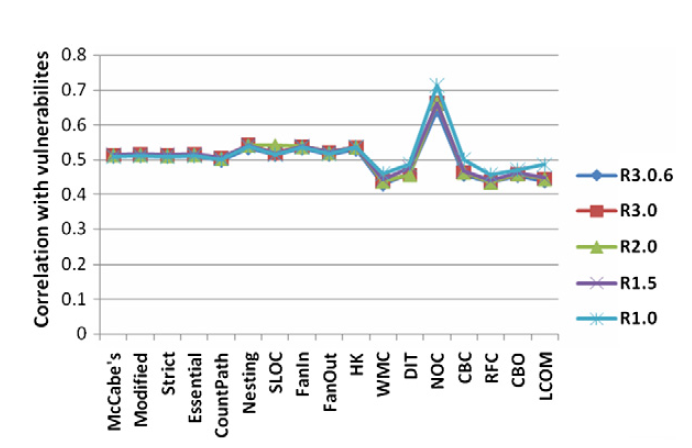
\includegraphics[width=\textwidth]{img/vulnerability_correlations.png}
	\caption{Korrelationen mit Sicherheitslücken zu verschiedenen Metriken~\cite{chowdhury_zulkernine_2009}.}
	\label{fig:correlations}
\end{figure}
Abbildung \ref{fig:correlations} zeigt die Korrelation mit Sicherheitslücken zu verschiedenen Metriken~\cite{chowdhury_zulkernine_2009}.
Die Linien zeigen verschiedene Release-Versionen von Mozilla Firefox.
Es lässt sich erkennen, dass die Korrelationsmuster über Versionen hinweg konsistent sind\cite{chowdhury_zulkernine_2009}.

\subsection{Klassifikatoren}
Mithilfe der Metriken lassen sich auch Klassifikatoren (englisch: \emph{predictors}) erstellen.
Der Ansatz basiert auf bereits bekannte Korrelationen aus vorherigen Forschungsergebnissen (siehe \ref{sec:ergebnisse}).
Er wird in \cite{chowdhury_zulkernine_2009} verwendet, um ein Framework für die Vorhersage von Sicherheitslücken zu entwickeln.
Abbildung \ref{fig:framework} zeigt die Architektur dieses Frameworks.
\begin{figure}
	\centering
	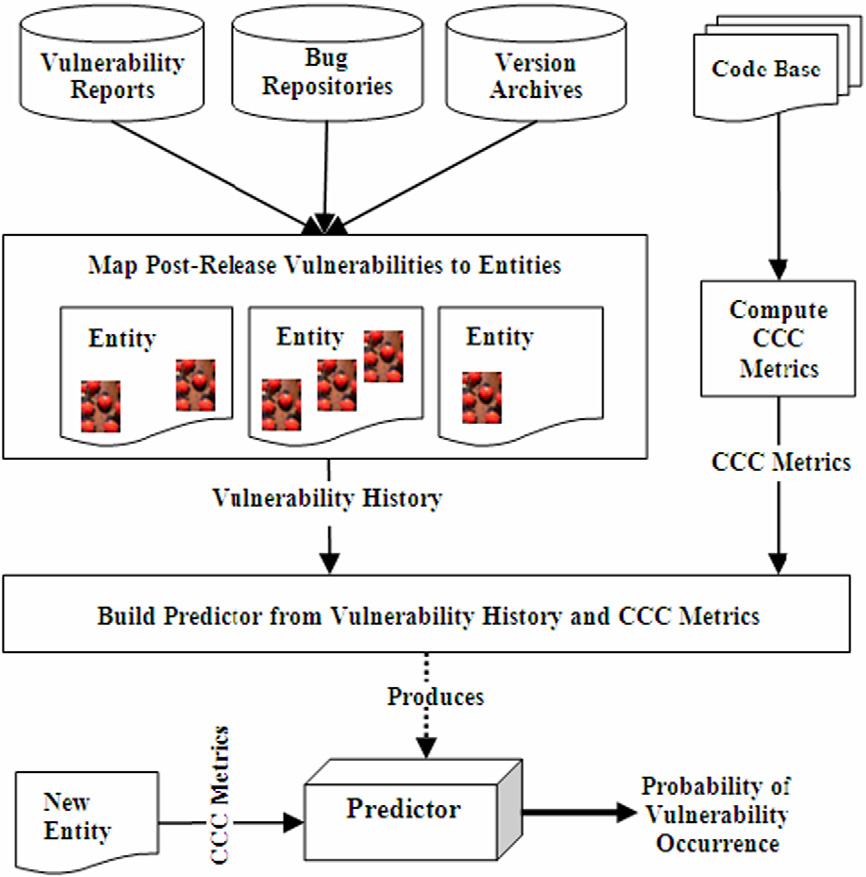
\includegraphics[width=0.7\textwidth]{img/framework.png}
	\caption{Framework für die Vorhersage von Sicherheitslücken aus \cite{chowdhury_zulkernine_2009}}
	\label{fig:framework}
\end{figure}
Die Herangehensweise unterscheidet sich dahingehend von der Berechnung der Korrelationen, dass die in anderen Studien festgestellte Korrelation der Metriken mit Sicherheitslücken nicht verwendet wurde, um Vorhersagen zu erstellen.

Das Problem wird als Klassifizierungsproblem auf Dateiebene aufgefasst:
Entweder eine Datei ist anfällig für Sicherheitslücken oder nicht.
Für die Klassifikatoren kommen verschiedene Techniken in Frage.
Beispiele sind \emph{Entscheidungsbäume}\cite{decision_trees}, die Weiterentwicklung \emph{Random Forests} und der \emph{Bayes Klassifikator}.
Für die Generierung der Klassifikatoren lässt sich die Bibliothek \emph{Waikato Environment for Knowledge Analysis (WEKA)}\footnote{WEKA Webseite: \url{https://www.cs.waikato.ac.nz/ml/weka/}} der Universität von Waikato, Neuseeland, verwenden~\cite{chowdhury_zulkernine_2009}.
Sie ist Open Source und in Java implementiert, sodass sie einfach und vielseitig eingesetzt werden kann.

Für die Generierung ist es notwendig, einen ausbalancierten Datensatz zu verwenden, um einseitige Klassifikatoren zu verhindern.
Anschließend können die Klassifikatoren generiert werden.
Ein Verfahren dafür ist \emph{Cross Validation}\cite{chowdhury_zulkernine_2009}.
Der Datensatz wird in 10 "`Bins"' aufgeteilt, wovon 9 zum Trainieren des Klassifikators und einer zum Testen der Vorhersagen benutzt werden.
Dieser Vorgang wird einige Male wiederholt.

Die generierten Klassifikatoren müssen anschließend noch auf ihre Qualität überprüft werden.
Chowdhury und Zulkernine verwenden dafür die Maße \emph{Accuracy}, \emph{Recall} und \emph{FN rate}~\cite{chowdhury_zulkernine_2009}.
Accuracy drückt aus, wie oft der Klassifikator die richtige Entscheidung getroffen hat.
Recall drückt aus, wie viele der Sicherheitslücken erkannt wurden.
Die FN Rate drückt aus, wie viele der Sicherheitslücken nicht erkannt wurden.
Sie werden auf folgende Weise berechnet:
\begin{equation}
	Accuracy = \frac{TP+TN}{TP+FP+TN+FN}
\end{equation}
\begin{equation}
	Recall = \frac{TP}{TP+FN}
\end{equation}
\begin{equation}
	FN rate = \frac{FN}{TP+FN}
\end{equation}
Dabei ist \emph{TP} (true positives) die Anzahl der korrekt erkannten Sicherheitslücken,
\emph{TN} (true negatives) die Anzahl der korrekt als ohne Lücke erkannten Dateien,
\emph{FP} (false positives) die Anzahl der fälschlicherweise erkannten Sicherheitslücken und
\emph{FN} (false negatives) die Anzahl der nicht erkannten Sicherheitslücken.
